

\tikzset{every picture/.style={line width=0.75pt}} %set default line width to 0.75pt

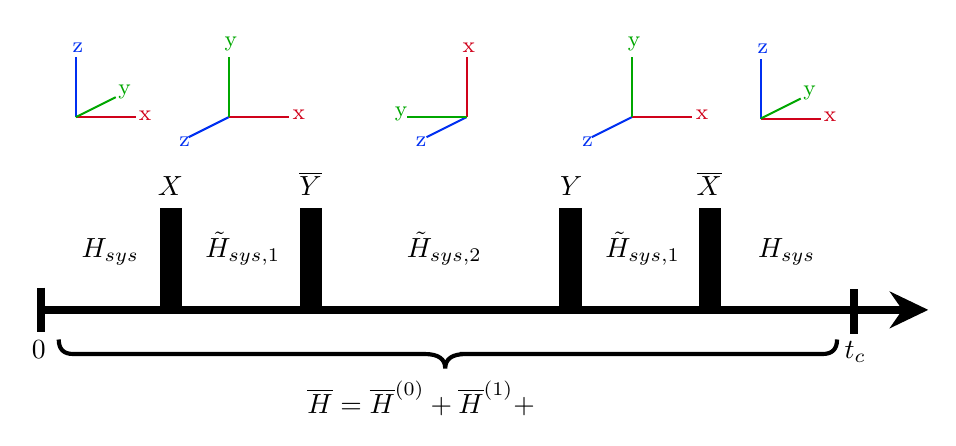
\begin{tikzpicture}[x=0.75pt,y=0.75pt,yscale=-1,xscale=1]
%uncomment if require: \path (0,214); %set diagram left start at 0, and has height of 214

%Shape: Rectangle [id:dp757529732417089]
\draw  [fill={rgb, 255:red, 0; green, 0; blue, 0 }  ,fill opacity=1 ] (70.71,95) -- (80.34,95) -- (80.34,144.35) -- (70.71,144.35) -- cycle ;
%Straight Lines [id:da8398663533091074]
\draw [line width=3]    (12.92,143.58) -- (434.5,143.58) ;
\draw [shift={(440.5,143.58)}, rotate = 180] [fill={rgb, 255:red, 0; green, 0; blue, 0 }  ][line width=0.08]  [draw opacity=0] (18.75,-9.01) -- (0,0) -- (18.75,9.01) -- (12.45,0) -- cycle    ;
%Shape: Rectangle [id:dp8989097393091372]
\draw  [fill={rgb, 255:red, 0; green, 0; blue, 0 }  ,fill opacity=1 ] (138.13,95) -- (147.76,95) -- (147.76,144.35) -- (138.13,144.35) -- cycle ;
%Shape: Rectangle [id:dp5203891268410358]
\draw  [fill={rgb, 255:red, 0; green, 0; blue, 0 }  ,fill opacity=1 ] (263.33,95) -- (272.96,95) -- (272.96,144.35) -- (263.33,144.35) -- cycle ;
%Shape: Rectangle [id:dp5922766644502158]
\draw  [fill={rgb, 255:red, 0; green, 0; blue, 0 }  ,fill opacity=1 ] (330.75,95) -- (340.38,95) -- (340.38,144.35) -- (330.75,144.35) -- cycle ;
%Shape: Brace [id:dp004729490444473794]
\draw  [line width=1.5]  (21.59,157.84) .. controls (21.59,162.51) and (23.92,164.84) .. (28.59,164.84) -- (197.8,164.84) .. controls (204.47,164.84) and (207.8,167.17) .. (207.8,171.84) .. controls (207.8,167.17) and (211.13,164.84) .. (217.8,164.84)(214.8,164.84) -- (389.57,164.84) .. controls (394.24,164.84) and (396.57,162.51) .. (396.57,157.84) ;
%Straight Lines [id:da5692356671850871]
\draw [color={rgb, 255:red, 208; green, 2; blue, 27 }  ,draw opacity=1 ]   (29.78,50.73) -- (58.68,50.73) ;
%Straight Lines [id:da6810769300954256]
\draw [color={rgb, 255:red, 0; green, 47; blue, 241 }  ,draw opacity=1 ]   (29.78,50.73) -- (29.78,21.84) ;
%Straight Lines [id:da050165915493954216]
\draw [color={rgb, 255:red, 0; green, 167; blue, 0 }  ,draw opacity=1 ]   (29.78,50.73) -- (49.05,41.1) ;

%Straight Lines [id:da5081204556289702]
\draw [color={rgb, 255:red, 208; green, 2; blue, 27 }  ,draw opacity=1 ]   (103.45,50.73) -- (132.35,50.73) ;
%Straight Lines [id:da6854547629628449]
\draw [color={rgb, 255:red, 0; green, 47; blue, 241 }  ,draw opacity=1 ]   (103.45,50.73) -- (84.19,60.36) ;
%Straight Lines [id:da7186146502407351]
\draw [color={rgb, 255:red, 0; green, 167; blue, 0 }  ,draw opacity=1 ]   (103.45,50.73) -- (103.45,21.84) ;

%Straight Lines [id:da24563094299910881]
\draw [color={rgb, 255:red, 208; green, 2; blue, 27 }  ,draw opacity=1 ]   (218.07,50.73) -- (218.07,21.84) ;
%Straight Lines [id:da179977702531384]
\draw [color={rgb, 255:red, 0; green, 47; blue, 241 }  ,draw opacity=1 ]   (218.07,50.73) -- (198.8,60.36) ;
%Straight Lines [id:da7516580599441232]
\draw [color={rgb, 255:red, 0; green, 167; blue, 0 }  ,draw opacity=1 ]   (218.07,50.73) -- (189.17,50.73) ;

%Straight Lines [id:da5137007458732086]
\draw [line width=3]    (404.72,133.57) -- (404.72,155.14) ;
%Straight Lines [id:da9300296101367684]
\draw [line width=3]    (12.92,132.8) -- (12.92,154.37) ;
%Straight Lines [id:da0881233734207878]
\draw [color={rgb, 255:red, 208; green, 2; blue, 27 }  ,draw opacity=1 ]   (359.79,51.4) -- (388.69,51.4) ;
%Straight Lines [id:da9374652913281989]
\draw [color={rgb, 255:red, 0; green, 47; blue, 241 }  ,draw opacity=1 ]   (359.79,51.4) -- (359.79,22.51) ;
%Straight Lines [id:da610003280154453]
\draw [color={rgb, 255:red, 0; green, 167; blue, 0 }  ,draw opacity=1 ]   (359.79,51.4) -- (379.06,41.77) ;

%Straight Lines [id:da5081271261395761]
\draw [color={rgb, 255:red, 208; green, 2; blue, 27 }  ,draw opacity=1 ]   (297.7,50.73) -- (326.59,50.73) ;
%Straight Lines [id:da9429921450367487]
\draw [color={rgb, 255:red, 0; green, 47; blue, 241 }  ,draw opacity=1 ]   (297.7,50.73) -- (278.43,60.36) ;
%Straight Lines [id:da28825440756966425]
\draw [color={rgb, 255:red, 0; green, 167; blue, 0 }  ,draw opacity=1 ]   (297.7,50.73) -- (297.7,21.84) ;


% Text Node
\draw (75.42,83.72) node  [font=\normalsize] [align=left] {$\displaystyle X$};
% Text Node
\draw (142.84,82.76) node  [font=\normalsize] [align=left] {$\displaystyle \overline{Y}$};
% Text Node
\draw (334.99,82.76) node  [font=\normalsize] [align=left] {$\displaystyle \overline{X}$};
% Text Node
\draw (268.53,83.72) node  [font=\normalsize] [align=left] {$\displaystyle Y$};
% Text Node
\draw (398.78,157.37) node [anchor=north west][inner sep=0.75pt]  [font=\normalsize]  {$t_{c}$};
% Text Node
\draw (7.12,156.98) node [anchor=north west][inner sep=0.75pt]  [font=\normalsize]  {$0$};
% Text Node
\draw (46.44,115.46) node  [font=\normalsize]  {$H_{\text{sys}}$};
% Text Node
\draw (110.29,114.02) node  [font=\normalsize]  {$\tilde{H}_{\text{sys, 1}}$};
% Text Node
\draw (207.38,114.02) node  [font=\normalsize]  {$\tilde{H}_{\text{sys, 2}}$};
% Text Node
\draw (302.92,114.02) node  [font=\normalsize]  {$\tilde{H}_{\text{sys, 1}}$};
% Text Node
\draw (372.27,115.46) node  [font=\normalsize]  {$H_{\text{sys}}$};
% Text Node
\draw (139.92,176.34) node [anchor=north west][inner sep=0.75pt]  [font=\normalsize]  {$\overline{H} =\overline{H}^{( 0)} +\overline{H}^{( 1)} +\dotsc $};
% Text Node
\draw (63.21,50.06) node  [font=\footnotesize,color={rgb, 255:red, 208; green, 2; blue, 27 }  ,opacity=1 ] [align=left] {x};
% Text Node
\draw (53.29,38.5) node  [font=\footnotesize,color={rgb, 255:red, 0; green, 167; blue, 0 }  ,opacity=1 ] [align=left] {y};
% Text Node
\draw (30.85,17.31) node  [font=\footnotesize,color={rgb, 255:red, 0; green, 47; blue, 241 }  ,opacity=1 ] [align=left] {z};
% Text Node
\draw (137.26,49.39) node  [font=\footnotesize,color={rgb, 255:red, 208; green, 2; blue, 27 }  ,opacity=1 ] [align=left] {x};
% Text Node
\draw (104.52,15.39) node  [font=\footnotesize,color={rgb, 255:red, 0; green, 167; blue, 0 }  ,opacity=1 ] [align=left] {y};
% Text Node
\draw (82.18,62.38) node  [font=\footnotesize,color={rgb, 255:red, 0; green, 47; blue, 241 }  ,opacity=1 ] [align=left] {z};
% Text Node
\draw (219.13,17.31) node  [font=\footnotesize,color={rgb, 255:red, 208; green, 2; blue, 27 }  ,opacity=1 ] [align=left] {x};
% Text Node
\draw (186.48,49.39) node  [font=\footnotesize,color={rgb, 255:red, 0; green, 167; blue, 0 }  ,opacity=1 ] [align=left] {y};
% Text Node
\draw (196.12,62.38) node  [font=\footnotesize,color={rgb, 255:red, 0; green, 47; blue, 241 }  ,opacity=1 ] [align=left] {z};
% Text Node
\draw (276.42,62.38) node  [font=\footnotesize,color={rgb, 255:red, 0; green, 47; blue, 241 }  ,opacity=1 ] [align=left] {z};
% Text Node
\draw (298.76,15.39) node  [font=\footnotesize,color={rgb, 255:red, 0; green, 167; blue, 0 }  ,opacity=1 ] [align=left] {y};
% Text Node
\draw (331.51,49.39) node  [font=\footnotesize,color={rgb, 255:red, 208; green, 2; blue, 27 }  ,opacity=1 ] [align=left] {x};
% Text Node
\draw (360.86,17.98) node  [font=\footnotesize,color={rgb, 255:red, 0; green, 47; blue, 241 }  ,opacity=1 ] [align=left] {z};
% Text Node
\draw (383.3,39.17) node  [font=\footnotesize,color={rgb, 255:red, 0; green, 167; blue, 0 }  ,opacity=1 ] [align=left] {y};
% Text Node
\draw (393.22,50.73) node  [font=\footnotesize,color={rgb, 255:red, 208; green, 2; blue, 27 }  ,opacity=1 ] [align=left] {x};


\end{tikzpicture}
